\documentclass{article}
\usepackage[utf8]{inputenc}
\usepackage{graphicx}
\usepackage{subcaption}
\usepackage{float}

\title{An Orthodontic Challenge}
\author{H. L. Eirew, B.D.S., L.D.S.}
\date{February 1976}

\begin{document}

\maketitle

This case report describes the orthodontic ‘‘decrowding’’ of a pair of identical twins, one by conventional extraction therefore, also therapy, the other by use of a function regulator.

The patient treated by appliance instead of extractions displayed a significantly better dental and facial result, and better long term prognosis.
Despite greater initial cost the more complex method may, prove economically superior.

The need for caution in premolar extraction procedures is stressed.
Wider use and study of facial photographic records seem essential in progressive orthodontic practice.

One of the most promising orthodontic developments of recent years has been Fraenkel’s discovery that moderate crowding of the dental arches may be relieved by the use of vestibular screen appliances instead of multiple premola: extractions.
Advantages arising from this procedure are:
\begin{enumerate}
\item Better dental arch form and appearance.
\item Better facial aesthetics.
\item Preservation of arch continuity and interdental contacts.
\item If there be still some arch length deficiency after treatment, remedial extractions may be confined to the molarregions without disturbance of arch integrity anteriorly.
This is particularly desirable in patients with deep overbite, threatened third molar problems or restriction of the nasal airway.
\end{enumerate}

A large number of cases of this type have been successfully treated by function regulator appliances at Fraenkel’s clinic in East Germany and described in various publications (Fraenkel, 1966, 1967, 1971, 1974).
Regrettably, supporting clinical material is still scarce in western countries and some scepticism has been expressed, even in well informed circles regarding the validity of this technique relative to the simpler and supposedly cheaper extraction procedure.

A unique opportunity for assessment of these conflicting views presented with the referral of a pair of identical twin sisters aged 12 years showing identical Class I malocclusions with overcrowding.
Their facial features and dental measurements were identical (Fig. 1A and B). Their family dentist had already extracted the deciduous canines of one sister and was about to repeat this measure for the other.
It was therefore decided to complete the extraction procedure in the first twin (E) in the customary manner with the removal of the first deciduous moiars and, later, the first premolars.

\begin{figure}[H]
    \centering
    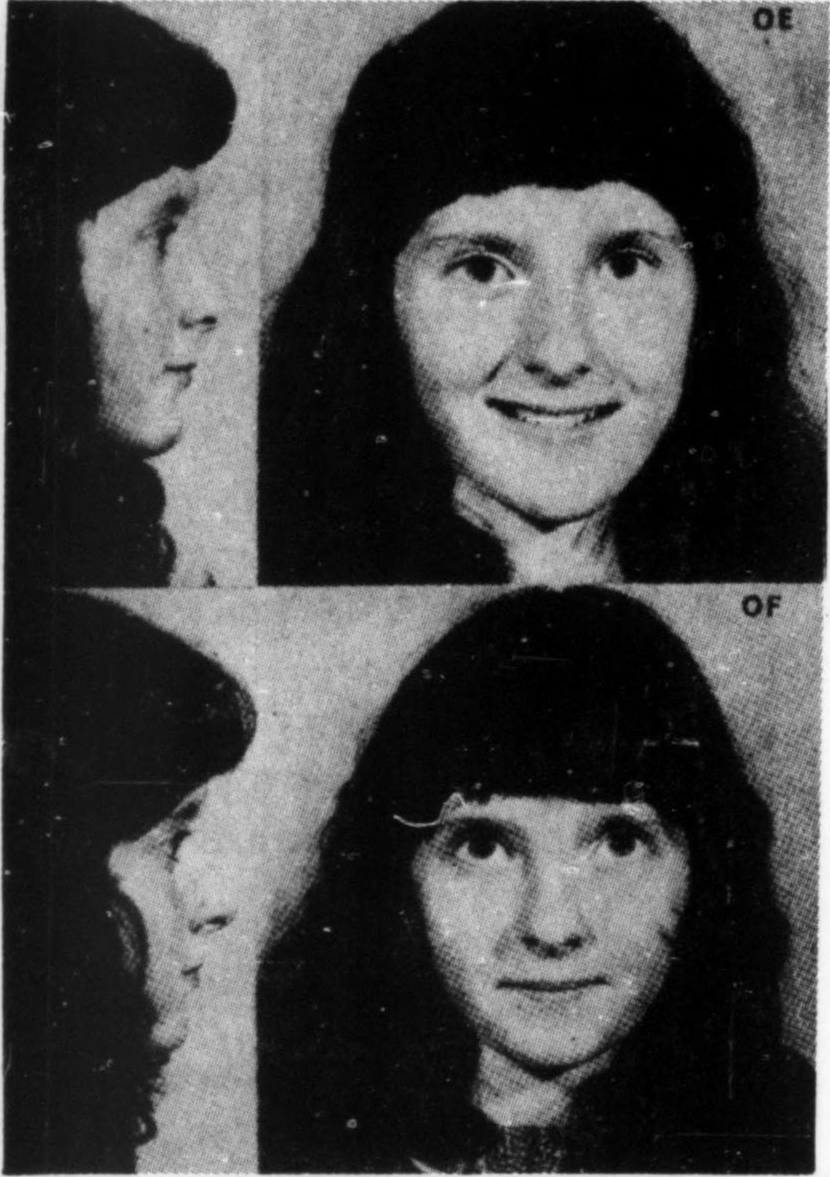
\includegraphics[width=0.5\linewidth]{fig01a.png}\\
    (A)
    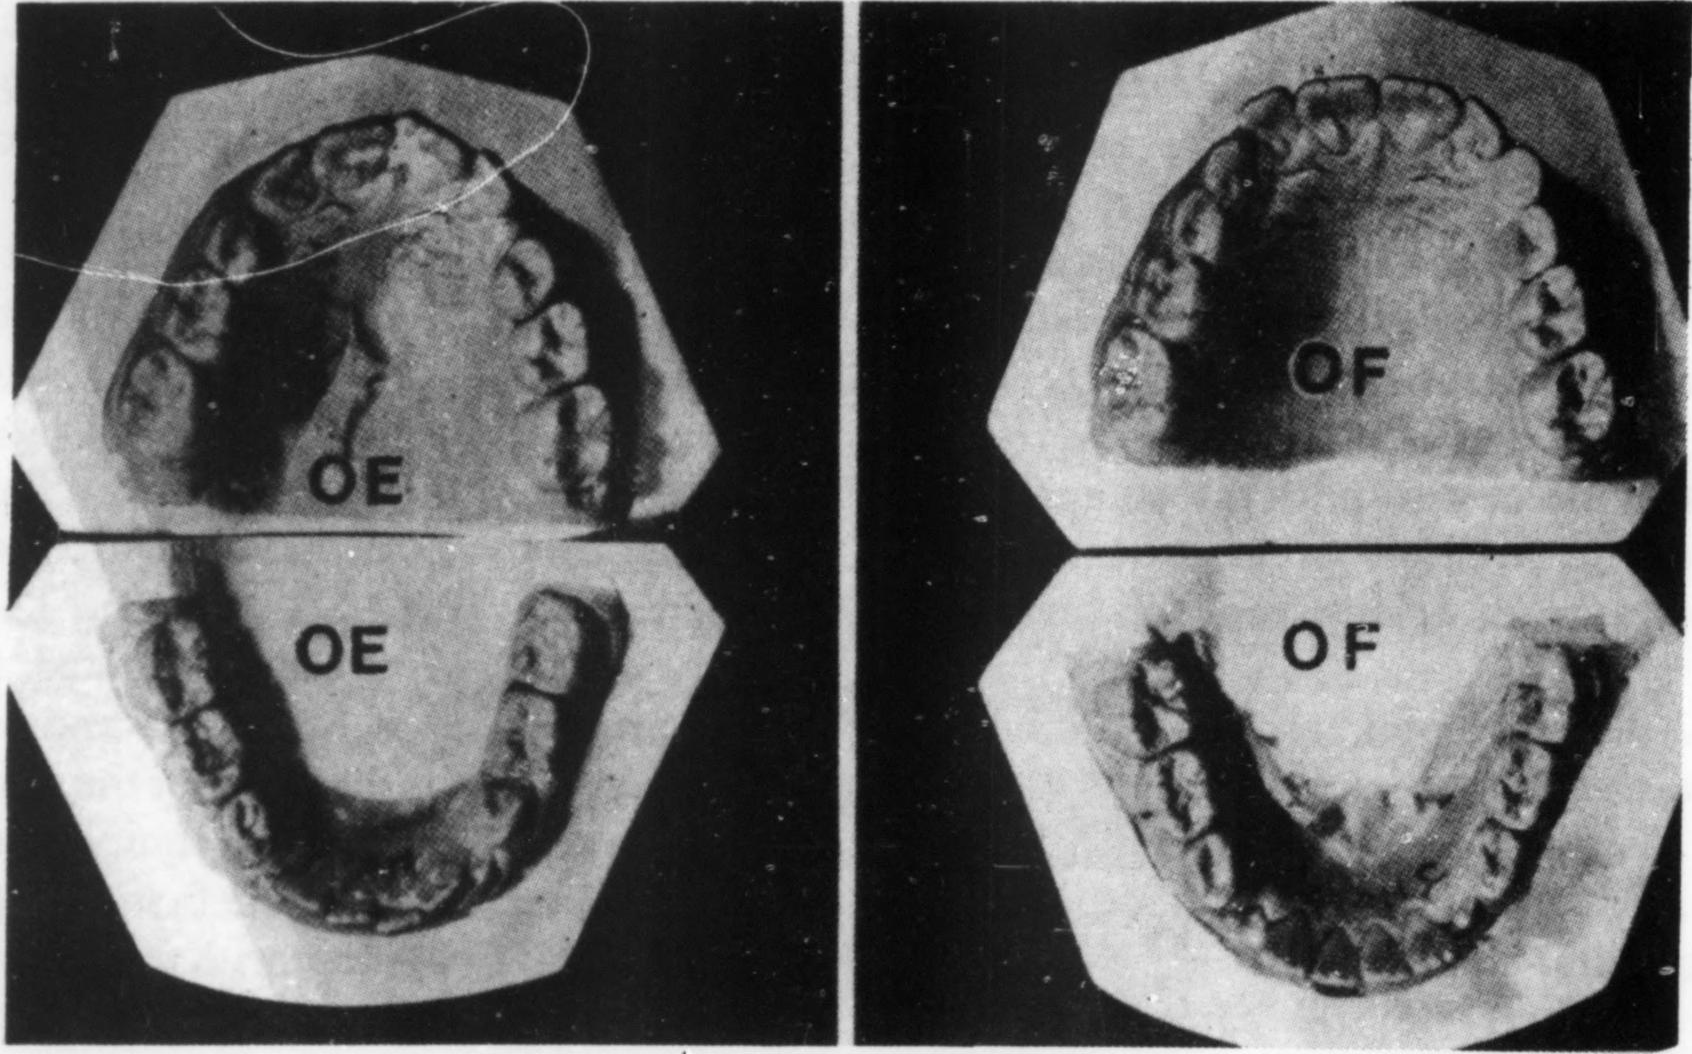
\includegraphics[width=0.95\linewidth]{fig01b.png}\\
    (B)
    \caption{A. Original appearance of twins; B, original models of twins.}
\end{figure}

As the dentition of the second twin (F) was still intact, it was decided to refrain from extractions but to treat her by the use of a Fraenkel appliance (type FR 1) for lateral arch development.

\section*{Clinical Findings}

Total treatment time in both cases was approximately 2 ½ years. The dental and facial changes of both twins during this period are shown in the illustrations.

Twin F (Fig. 2), treated by Fraenkel appliance, shows a pleasing round arch form.
The upper dental arch was widened by 4-5 mm. between the first premolars and by 2 mm. between the first molars.
Lower arch development was similar.
All round occlusion and interdental contact are perfect.
The incisor bite has been opened by 2 mm. The prognosis for good dental health and longevity of the dentition seems excellent.

\begin{figure}[H]
\centering
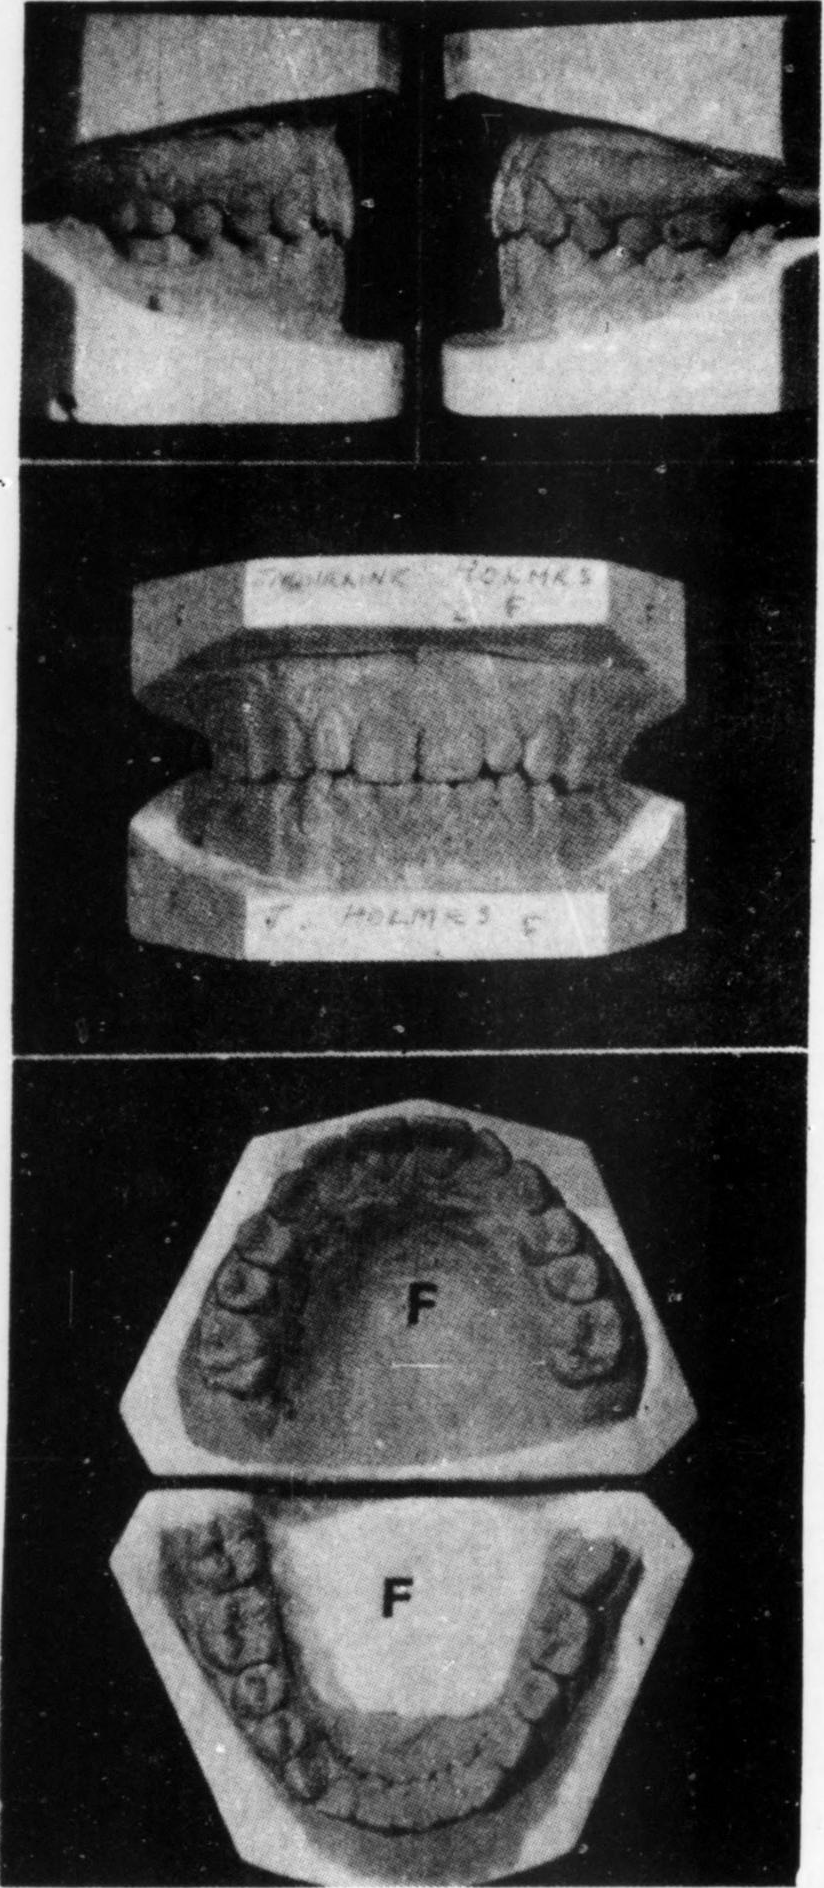
\includegraphics[width=0.5\linewidth]{fig02.png}
\caption{Final models of twin treated by function regulator appliance without extractions.}
\end{figure}

Facially the girl is good looking, with a rounded facial form matching her attractive rounded dental arch.
She is happy with the result of her orthodontic treatment and considers the effort to wear the appliance well rewarded (Fig. 3).

\begin{figure}[H]
    \centering
    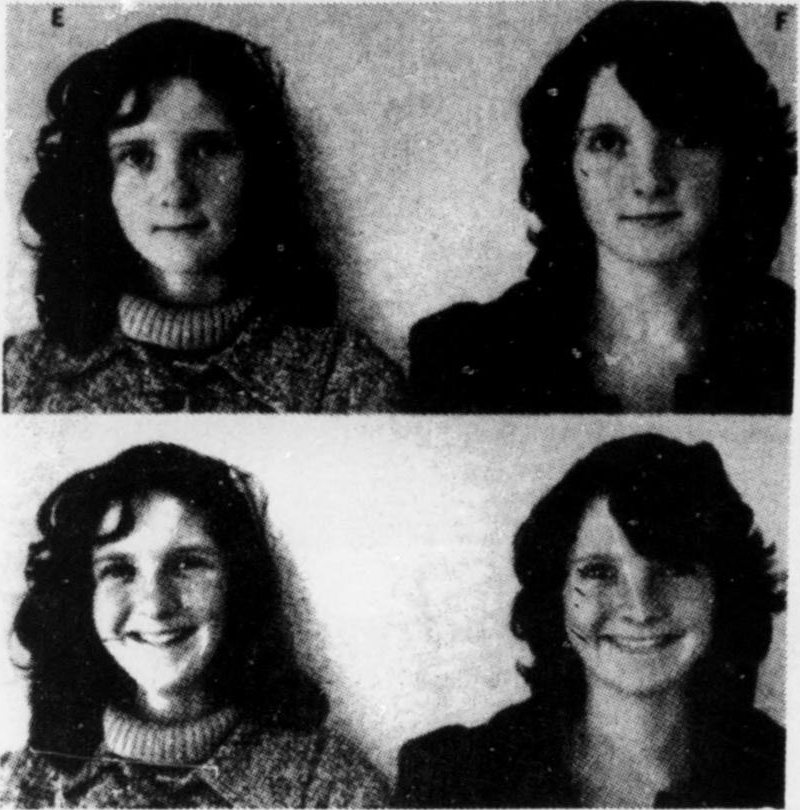
\includegraphics[width=0.5\linewidth]{fig03.png}
    \caption{Post-treatment appearance of twins.}
\end{figure}

Twin E (Fig. 4), treated by extractions, shows some relief of crowding and of incisal irregularity.
She still has a tapering archform accentuated by narrow arch width.
There has been no lateral development.
Residual extraction spaces are still visible after more than three years.
The cheek teeth have slipped out of correct occlusion and contact on both sides.
The deep bite persists.
Dental arch appearance is poor.
The lack of arch continuity and of good contacts implies a considerable hazard to dental and periodontal health in the long term.

\begin{figure}[H]
    \centering
    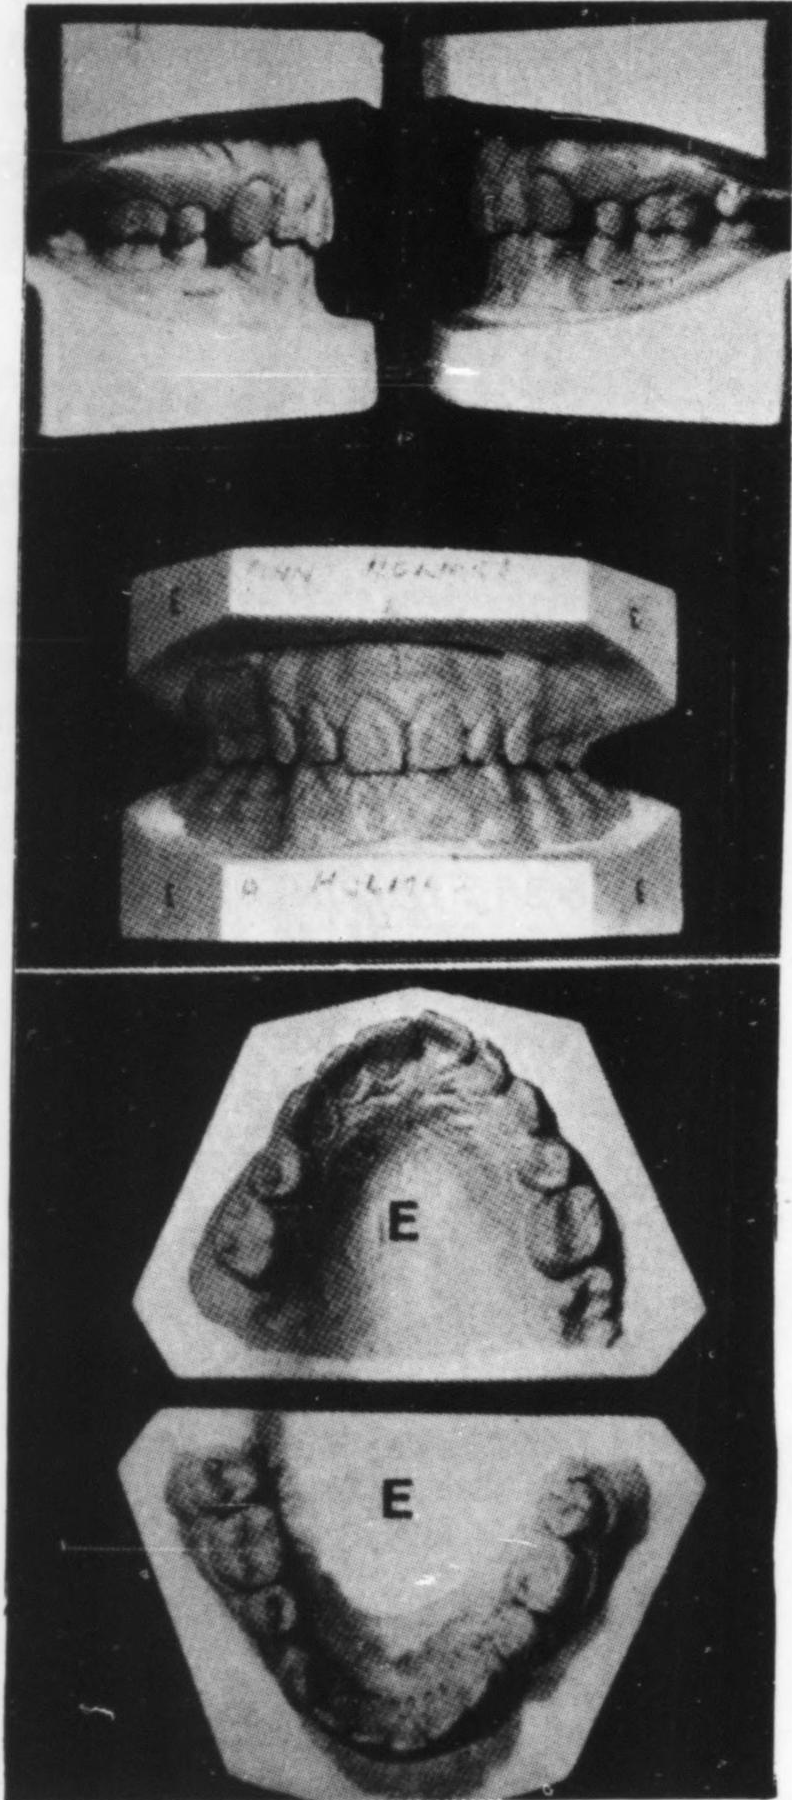
\includegraphics[width=0.5\linewidth]{fig04.png}
    \caption{Final models of twin treated by extractions only.}
\end{figure}

Her facial deterioration has been quite disasterous.
In the years from 12 to 14 she has become a ‘little old woman’ in relation to her sister.
The changes shown resemble those seen in the elderly when bone resorption follows multiple tooth loss.
As her general health and dietary habits are normal and resemble those of her sister, the facial change seems only attributable to lack of skeletal development following the extractions.

Most distressing of all is the emotional effect on the patient.
She is acutely aware of the marked difference in appearance between herself and her sister and has developed a considerable inferiority complex.
She feels that fate has dealt her a very unkind blow, making her the ‘ugly sister’.
This reaction has now become so disturbing that further investigation has been discontinued. Obviously, no form of orthodontic appliance therapy can remedy the skeletal and facial damage.

\section*{Discussion}

These findings raise a number of important points; general dental, orthodontic, aesthetic, psychological, social and economic aspects are worthy of consideration.

The treatment by Fraenkel appliance proved entirely satisfactory and the cost was relatively modest.
The outcome is ahappy, satisfied patient with a dentition likely to make minimal demands in the forseeable future.

The extraction treatment of the other twin satisfies only the most uncritical requirements and the questionable concept of ‘doing most for the largest number of patients, given limited financial resources’.
An acceptable plaster model result has been achieved and in due course some further space closure and spontaneous incisor alinement might be expected.
In every other respect — dental, facial and psychological — the result is unacceptable.
The cost of her treatment was less than that of her sister’s appliance treatment, but not markedly, as three extraction sessions — with general anaesthetics administered by a consultant — were required.
Her future dental treatment needs cannot be foreseen, but the prognosis seems much less favourable than in her sister’s case.
Even in the medium term, any economics achieved may therefore prove illusory.

The findings in this pair of identical twins support the observations reported by Fraenkel and his co-workers.
They call into question the widely held belief in a genetically predetermined, unalterable dento-facial growth pattern. It would seem that by their differential treatment, the developmental pattern of twin F was influenced favourably, the pattern of twin E adversely.

But for the existence of an identical twin for comparison, the facial deterioration of twin E might never have been noted at all or dismissed as a normal feature of ‘growing up’.
Even so, the full measure of the differential reaction of the two patients could only be assessed by means of photographic records.
Overcrowding is the most common form of malocclusion and in this country some thousands of children every year are treated by premolar extraction procedures, with or without appliance therapy.
In the case of twin E it might be argued that it would have been better if she had received no intervention at all rather than the much used measure chosen.
This is no solid evidence to indicate that her adverse response is matched by all or indeed many patients subjected to premolar extractions in similar circumstances, but personal impression suggests that this is not an infrequent reaction.
It is therefore to be feared, that numbers of patients may have suffered permanent facial damage in the course of simple orthodontic treatment.

\section*{Conclusions}

It would appear that much remains to be learned about the effect of extractions on dento-facial development.
The necessary knowledge will only be gained by the study of long term facial photographic records of children receiving orthodontic treatment by diverse techniques, with and without extractions, and of similar control groups.

It is suggested that in our present state of knowledge non-extraction or molar extraction procedures should receive preference whenever possible, except in mono- or bi-maxillary protrusion cases where a reduction of anterior arch material appears clearly indicated.

P.S. Two points that do not emerge from the original article are:
\begin{enumerate}
\item The identity of the twins was confirmed by full haematological investigation.
\item Both patients were submitted for treatment to the British National Health Service, but were refused appliance therapy, it being considered that their requirement could be satisfied by remedial extractions only.
\end{enumerate}

\raggedleft
H.L. Eirew, B.D.S., L.D.S. \\
Withington, Manchester, England \\
\raggedright

\section*{References}
\begin{itemize}
\item Fraenkel, R.: Trans. Europ. Orthodont. Soc., p- 233, 1966.
\item Fraenkel, R.: Funktionskieferorthopaedie und der Mundvorhof als apparative Basis. Verlag Volk und Gesundheit, Berlin, 1967.
\item Fraenkel, R.: Trans. Europ. Orthodont. Soc., p- 303, 1971.
\item Fraenkel, R.: Amer. J. Orthodont., 65: 372, 1974.
\end{itemize}

\end{document}